\documentclass{article}

\usepackage{amsmath}
\usepackage{dsfont}
\usepackage{geometry}
\usepackage{graphicx}

\geometry{left=1.5cm, right=1.5cm, top=2cm, bottom=2cm}

\title{Preferential Attachment Model Modifications}
\author{Karol Janic}
\date{\today}

\begin{document}

\maketitle

\section*{Preferential Attachment with Probabilistic Acceptance}

\subsection*{Model description}
\begin{enumerate}
    \item start with cycle/clique of $n_0$ nodes and $m_0$ edges
    \item add a new node
    \item select $m$ existing nodes (without last added node) with probability proportional to their degree
    \item for each selected node, accept the connection with probability $p$
    \item if no connections were made, remove the new added node
    \item repeat from steps 2-5 $n$ times
\end{enumerate}

\subsection*{Final number of nodes - expected number and variance}
\begin{equation}
    E[N] = n_0 + n \cdot (1 - (1 - p)^m)
\end{equation}
\textbf{Comment:} The expected number of accepted nodes follows a binomial distribution with parameters $n$ and $1 - (1 - p)^m$. 
Adding the initial $n_0$ nodes gives the total expected number of nodes.

\begin{equation}
    Var[N] = n \cdot (1 - (1 - p)^m) \cdot (1 - p)^m
\end{equation}
\textbf{Proof:} The variance of the number of accepted nodes follows a binomial distribution with parameters $n$ and $1 - (1 - p)^m$.

\subsection*{Final number of edges - expected number and variance}
\begin{equation}
    E[E] = m_0 + n \cdot m \cdot p
\end{equation}
\textbf{Comment:} Each new node attempts to create $m$ edges, each accepted with probability $p$. Thus, the expected number of edges added per new node is $m \cdot p$. Adding the initial $m_0$ edges gives the total expected number of edges.

\begin{equation}
    Var[E] = n \cdot m \cdot p \cdot (1 - p)
\end{equation}
\textbf{Proof:} The number of edges added by each new node follows a binomial distribution with parameters $m$ and $p$. Thus, the variance of the number of edges added per new node is $m \cdot p \cdot (1 - p)$.

\subsection*{Degree dynamics}
Let $k_i(t)$ be the degree of node $i$ at time $t \geq i$.

\begin{equation}
    \frac{dk_i}{dt} = \frac{k_i(t)}{\sum_{j} k_j(t)} \cdot m \cdot p = \frac{k_i(t) \cdot m \cdot p}{2 \cdot (m_0 + m \cdot p \cdot t)} = \frac{k_i(t)}{2 \cdot (\frac{m_0}{m \cdot p} + t)}
\end{equation}
\begin{equation}
    \frac{dk_i}{dk} = \frac{dt}{2 \cdot (\frac{m_0}{m \cdot p} + t)} \implies 
    \int_{k_i(i) = m \cdot p}^{k_i(t)} \frac{1}{k}\, dk \;=\; \int_{i}^{t} \frac{1}{2 \cdot (\frac{m_0}{m \cdot p} + t')}\, dt'
\end{equation}
\begin{equation}
    \ln\!\big(k_i(t)\big) - \ln(m \cdot p) \;=\; \tfrac{1}{2}\big(\ln(\frac{m_0}{m \cdot p} + t) - \ln(\frac{m_0}{m \cdot p} + i)\big)
\end{equation}
\begin{equation}
    k_i(t) \;=\; m \cdot p \cdot \exp\!\big(\tfrac{1}{2}(\ln(\frac{m_0}{m \cdot p} + t) - \ln(\frac{m_0}{m \cdot p} + i))\big) \;=\; m \cdot p \cdot \sqrt{\frac{\frac{m_0}{m \cdot p} + t}{\frac{m_0}{m \cdot p} + i}}
\end{equation}
For large enough $t$:
\begin{equation}
    k_i(t) \;=\; m \cdot p \cdot \sqrt{\frac{t}{i}}
\end{equation}


\subsection*{Max degree}
The maximum degree $k_{max}$ can be estimated by considering the oldest node (node 1) at time $t = n$:
\begin{equation}
    k_{max} \approx k_1(n) = m \cdot p \cdot \sqrt{n}
\end{equation}

\subsection*{The most common degree}
The most common degree $k^*$ can be estimated by finding the mode of the initial degree distribution $B(m, p)$:
\begin{equation}
    \lceil m \cdot p \rceil \geq k^* \geq \lfloor m \cdot p \rfloor
\end{equation}

\subsection*{Degree distribution}
Initial node degree $k_t$ at time $t$ follows binomial distribution $B(m, p)$:
\begin{equation}
    s_k = P(k_t = k) = \binom{m}{k} \cdot p^k \cdot (1 - p)^{m - k}, \quad k = 0, 1, \ldots, m
\end{equation}
Let $p_k(t)$ be the probability that a randomly chosen node has degree $k$ at time $t$ and $N_k(t)$ be the number of nodes with degree $k$ at time $t$. Then:
\begin{equation}
    N_k(t+1) - N_k(t) = \frac{k - 1}{2(m_0 + m  \cdot  p  \cdot t)} \cdot m \cdot p \cdot N_{k - 1}(t) - \frac{k}{2(m_0 + m  \cdot  p  \cdot t)} \cdot m \cdot p \cdot N_k(t) + s_k
\end{equation}
\begin{equation}
    (t+1) \cdot p_k(t+1) - t \cdot p_k(t) = \frac{k - 1}{2(m_0 + m  \cdot  p  \cdot t)} \cdot m \cdot p \cdot t \cdot p_{k - 1}(t) - \frac{k}{2(m_0 + m  \cdot  p  \cdot t)} \cdot m \cdot p \cdot t \cdot p_k(t) + s_k
\end{equation}
\begin{equation}
    p_k(t+1) = \frac{k - 1}{2(\frac{m_0}{m \cdot p \cdot t} + 1)} \cdot p_{k - 1}(t) - \frac{k}{2(\frac{m_0}{m \cdot p \cdot t} + 1)} \cdot p_k(t) + s_k
\end{equation}
For large enough $t$, we can approximate $p_k(t+1) = p_k(t)$:
\begin{equation}
    p_k(t) = \frac{k - 1}{2(\frac{m_0}{m \cdot p \cdot t} + 1)} \cdot p_{k - 1}(t) - \frac{k}{2(\frac{m_0}{m \cdot p \cdot t} + 1)} \cdot p_k(t) + s_k    
\end{equation}
\begin{equation}
    \!\big(1+ \frac{k}{\frac{m_0}{m \cdot p \cdot t} + 1}\big) \cdot p_k(t) = \frac{k - 1}{\frac{m_0}{m \cdot p \cdot t} + 1} \cdot p_{k - 1}(t) + 2s_k
\end{equation}
Let $a = \frac{m_0}{m \cdot p \cdot t} + 1$, then:
\begin{equation}
    p_k(t) = \frac{k-1}{k + 2 \cdot a} \cdot p_{k - 1}(t) + \frac{2 \cdot a}{k + 2 \cdot a} \cdot s_k
\end{equation}
For large enough $t$, $a \approx 1$:
\begin{equation}
    p_k(t) = \frac{k-1}{k + 2} \cdot p_{k - 1}(t) + \frac{2}{k + 2} \cdot s_k
\end{equation}

% \textbf{Comment:} 
% \begin{itemize}
%     \item The term $\frac{k-1}{2(m_0 + m \cdot p \cdot t)} \cdot m \cdot p \cdot N_{k-1}(t)$ represents the expected number of nodes that will increase their degree from $k-1$ to $k$ due to the addition of a new node.
%     \item The term $\frac{k}{2(m_0 + m \cdot p \cdot t)} \cdot m \cdot p \cdot N_k(t)$ represents the expected number of nodes that will increase their degree from $k$ to $k+1$ due to the addition of a new node.
%     \item The term $s_k$ represents the expected number of new nodes that are added with degree $k$.
% \end{itemize}

\subsection*{Explicit solution for degree distribution - simple case}
\begin{equation}
    p_k = \frac{2}{k(k+1)(k+2)} \sum_{j=0}^{\min(k,m)} j \cdot (j+1) \cdot s_j
\end{equation}

\subsection*{Explicit solution for degree distribution - general case}
\begin{equation}
    p_k = \frac{(k-1)!}{\Gamma(2a+k+1)} \sum_{j=1}^{k} \frac{2a \cdot \Gamma(2a+j)}{(j-1)!} \cdot s_j
\end{equation}

\newpage

\section*{Log Based Preferential Attachment}

\subsection*{Model description}
\begin{enumerate}
    \item start with cycle/clique of $n_0$ nodes and $m_0$ edges
    \item add a new node
    \item select $m$ existing nodes (without last added node) with probability proportional to $\log(d + 1)$, where $d$ is the degree of the node
    \item connect to all selected nodes
    \item repeat from steps 2-4 $n$ times
\end{enumerate}

\subsection*{Degree dynamics}
Let $S(t) = \sum_{j=1}^t \log(k_j(t) + 1)$.
\begin{equation}
    S(t) = \sum_{j=1}^t \log(k_j(t) + 1) \geq \sum_{j=1}^t \log(m + 1) = t \cdot \log(m + 1)
\end{equation}
\begin{equation}
    S(t) = \sum_{j=1}^t \log(k_j(t) + 1) = t \cdot \sum_{j=1}^t \frac{1}{t} \log(k_j(t) + 1) \leq t \cdot \log(\frac{1}{t} \sum_{j=1}^t (k_j(t) + 1)) = t \cdot \log(\frac{2 \cdot (m_0 + m \cdot t) + t}{t})
\end{equation}
For $t \geq 2 \cdot m_0$:
\begin{equation}
    t \cdot \log(m + 1) \leq S(t) \leq t \cdot \log(2m + 2) = t \cdot \log(2(m + 1)) = t \cdot (\log 2 + \log(m + 1))
\end{equation}
\newline
Let $k_i(t)$ be the degree of node $i$ at time $t \geq i$.
\begin{equation}
    \frac{dk_i}{dt} = \frac{\log(k_i(t) + 1)}{\sum_{j} \log(k_j(t) + 1)} \cdot m = \frac{\log(k_i(t) + 1)}{S(t)} \cdot m
\end{equation}
\begin{equation}
    \frac{dk_i}{log(k_i(t) + 1)} = \frac{m}{log(m+1)} \cdot \frac{1}{t} \cdot dt \implies
    \int_{k_i(i) = m}^{k_i(t)} \frac{1}{\log(k + 1)}\, dk \;=\; \frac{m}{\log(m+1)} \int_{i}^{t} \frac{1}{t'}\, dt'
\end{equation}
\begin{equation}
    Li(\log(k_i(t) + 1)) - Li(\log(m + 1)) \;=\; \frac{m}{\log(m+1)} (\log(t) - \log(i)) = \frac{m}{\log(m+1)} \log(\frac{t}{i})
\end{equation}
\begin{equation}
    k_i(t) \;=\; \exp(Li^{-1}(Li(\log(m + 1)) + \frac{m}{\log(m+1)} \log(\frac{t}{i}))) - 1
\end{equation}
\begin{equation}
    ...
\end{equation}

\subsection*{Max degree}
\begin{equation}
    ...
\end{equation}

\subsection*{Degree distribution}
\begin{equation}
    N_k(t+1) - N_k(t) = \frac{\log(k - 1 + 1)}{S(t)} \cdot m \cdot N_{k - 1}(t) - \frac{\log(k + 1)}{S(t)} \cdot m \cdot N_k(t) + s_k
\end{equation}
\begin{equation}
    (t+1) \cdot p_k(t+1) - t \cdot p_k(t) = \frac{\log(k)}{S(t)} \cdot m \cdot t \cdot p_{k - 1}(t) - \frac{\log(k + 1)}{S(t)} \cdot m \cdot t \cdot p_k(t) + s_k
\end{equation}
\begin{equation}
    p_k(t+1) = \frac{\log(k)}{S(t)} \cdot m \cdot t \cdot p_{k - 1}(t) - \frac{\log(k + 1)}{S(t)} \cdot m \cdot t \cdot p_k(t) + s_k
\end{equation}
\begin{equation}
    p_k(t) = \frac{\log(k)}{t \cdot log(m+1)} \cdot m \cdot t \cdot p_{k - 1}(t) - \frac{\log(k + 1)}{t \cdot log(m+1)} \cdot m \cdot t \cdot p_k(t) + s_k
\end{equation}
\begin{equation}
    p_k(t) \sim exp(C \cdot \frac{k}{log(k)})
\end{equation}

\newpage

\section*{Log Based Preferential Attachment with Probabilistic Acceptance}
This combination combines an exponential vertex degree distribution for degrees $>m$ and a specific distribution for degrees $\leq m$.
This model better fits biological network models. Example degree distributions:

\vspace{0.5cm}

\begin{figure}[h]
    \centering
    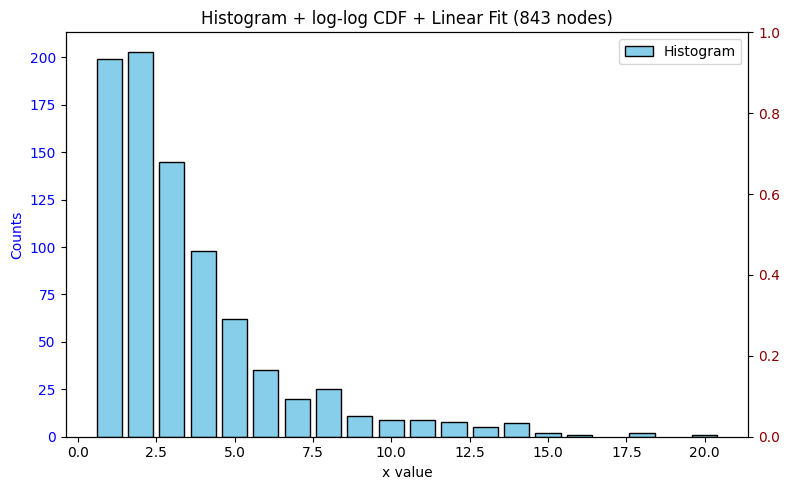
\includegraphics[width=0.6\textwidth]{example1.png}
    \caption{Example degree distribution for $m=5$, $p=0.3$, $n=1000$, $n_0=10$, $m_0=10$.}
\end{figure}
\vspace{0.5cm}

\begin{figure}[h]
    \centering
    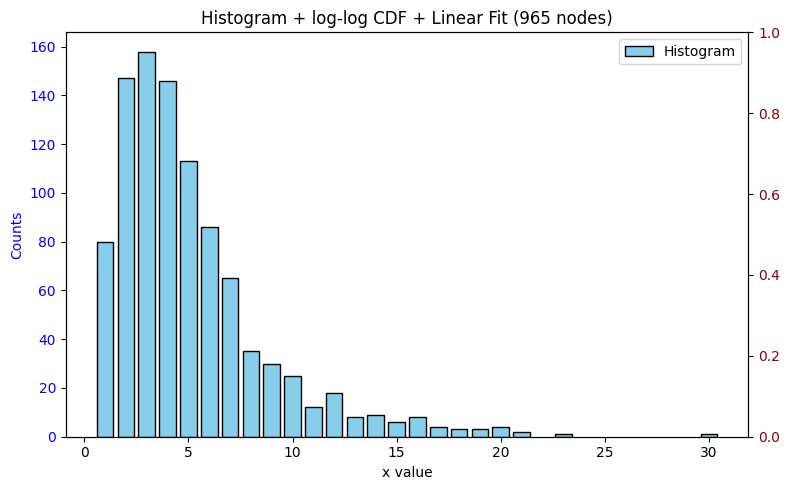
\includegraphics[width=0.6\textwidth]{example2.png}
    \caption{Example degree distribution for $m=5$, $p=0.5$, $n=1000$, $n_0=10$, $m_0=10$.}
\end{figure}

\newpage

\section*{Motifs counting in Variate Preferential Attachment Models}

\subsection*{Model description}
\begin{enumerate}
    \item start with single node with self-loop
    \item add a new node
    \item select existing node (without last added node) with probability proportional to $f(d)$, where $d$ is the degree of the node and $f$ is a given function
    \item connect to all selected nodes
    \item repeat from steps 2-4 $m \cdot n$ times
    \item merge consecutive $m$ added nodes into $n$ final nodes - each final node connects to all nodes connected to any of its merged nodes, looping edges and multiple edges are removed
\end{enumerate}

\subsection*{Mathematical model description}
Let's define random graph process $\{G_t\}_{t \geq 1}$, where $G_t = (V_t, E_t)$ is a graph at time $t$ with vertex set $V_t = \{1, 2, \ldots, t\}$ and edge set $E_t$.
Graph $G_{t+1}$ is obtained from $G_t$ by adding a new node $t+1$ and connecting it to an existing node $i \in V_t$ selected with probability proportional to $f(d_i(t))$, where $d_i(t)$ is the degree of node $i$ at time $t$.
\newline
\newline
The probability of selecting node $i$ at time $t$ is given by:
\begin{equation}
    \mathds{P}[i \text{ is selected at time } t+1] = \frac{f(d_i(t))}{\sum_{j=1}^{t} f(d_j(t))} = \phi_t(i)
\end{equation}

\subsection*{Motifs counting}
Let $S = (V_S, E_S)$ be a fixed motif graph with vertex set $V_S$ and edge set $E_S$. The probability $\mathds{P}[S \subseteq G_t]$ means the probability that motif $G_n$ contains exactly edge set $E_S$ among its edges.
\newline
\newline
Let $S_t = (V_{S_t}, E_{S_t})$ be the subgraph of $G_t$ induced by the first $t$ nodes - $\{1, 2, \ldots, t\}$.
\newline
\newline
Let $R_t(i)$ (for $t \geq i$) be number of edges in $S$ incoming to node $i$ from nodes added after time $t$. 
\newline
This means $R_t(i) = |\{(i,j) \in E_S : j > t\}|$.
\newline
\newline
Let define event $X_t$ - event that motif $S$ is contained in $G_t$.
\begin{equation}
    X_t = \prod_{(i,j) \in E_{S_t}} \mathds{1}_{(i,j) \in E_t} \cdot \prod_{i \in V_{S_t}, i \leq t} [d_t(i)]_{R_t(i)},
\end{equation}
where $\mathds{1}_{(i,j) \in E_t}$ is indicator function that is 1 if edge $(i,j)$ is in $E_t$ and 0 otherwise and $[d_t(i)]_{R_t(i)}$ is the rising factorial defined as:
\begin{equation}
    [d_t(i)]_{R_t(i)} = d_t(i) \cdot (d_t(i) + 1) \cdot (d_t(i) + 2) \cdots (d_t(i) + R_t(i) - 1). 
\end{equation}
\newline
Meaning of $X_t$:
\begin{itemize}
    \item the first product ensures that all edges in $E_{S_t}$ are present in $E_t$
    \item the second product ensures that for each node $i$ in $V_{S_t}$, there are enough edges incoming from nodes added after time $t$ to complete the motif, consecutively increasing the degree of node $i$ by $R_t(i)$ is responsible for selection of parent nodes for these incoming edges
\end{itemize}
The probability that motif $S$ is contained in $G_t$ is given by:
\begin{equation}
    \mathds{P}[S \subseteq G_t] = \mathds{E}[X_t]
\end{equation}

\newpage

\subsection*{Recursion for $X_t$ - adding $t+1$ node}
\begin{align}
    X_{t+1} &= R_{t+1}(t+1)! \cdot \prod_{(i,j) \in E_{S_{t+1}}} \mathds{1}_{(i,j) \in E_{t+1}} \cdot \prod_{i \in V_{S_t}, i \leq t} [d_{t+1}(i)]_{R_{t+1}(i)} = \\
            &= R_{t+1}(t+1)! \cdot Y
\end{align}
Where:
\begin{itemize}
    \item $R_{t+1}(t+1)!$ accounts for the ways to connect the new node $t+1$ to its required parents in motif $S$
    \item the first product ensures that all edges in $E_{S_{t+1}}$ are present in $E_{t+1}$
    \item the second product ensures that for each node $i$ in $V_{S_t}$, there are enough ways to connect incoming edges from nodes added after time $t+1$ to complete the motif
\end{itemize}

\subsubsection*{$S$ does not contain node edge ${(k, t+1)}$ for any $k \in V_{S_t}$}
Then:
\begin{itemize}
    \item $S_{t+1} = S_t$
    \item $R_{t+1}(t+1) = 0$ for all $i \leq t$
    \item $d_{t+1}(i) = d_t(i) + 1$ if node $i$ was selected at time $t+1$, otherwise $d_{t+1}(i) = d_t(i)$
\end{itemize}
So:
\begin{equation}
    Y   = \prod_{(i,j) \in E_{S_t}} \mathds{1}_{(i,j) \in E_{t}} \cdot \prod_{i \in V_{S_t}} [d_{t+1}(i)]_{R_t(i)}
\end{equation}
If node $i$ was selected at time $t+1$ - event with probability $\phi_t(i)$:
\begin{equation}
    [d_{t+1}(i)]_{R_t(i)} = [d_t(i) + 1]_{R_t(i)} = [d_t(i)]_{R_t(i)} \cdot \frac{d_t(i) + R_t(i)}{d_t(i)} = [d_t(i)]_{R_t(i)} \cdot \left(1 + \frac{R_t(i)}{d_t(i)}\right)
\end{equation}
Then:
\begin{equation}
    \mathds{E}[Y - X_t \mid G_t] = X_t \cdot \sum_{i \in V_{S_t}} \phi_t(i) \cdot \frac{R_t(i)}{d_t(i)} \\
\end{equation}
Then:
\begin{equation}
    \mathds{E}[X_{t+1} \mid G_t] = R_{t+1}(t+1)! \cdot \left(1 + \sum_{i \in V_{S_t}} \phi_t(i) \cdot \frac{R_t(i)}{d_t(i)}\right) \cdot X_t
\end{equation}
\newline
\subsubsection*{$S$ contains node edge ${(k, t+1)}$ for some $k \in V_{S_t}$}
We need edge ${(k, t+1)}$ to be present in $E_{t+1}$, which happens only if node $k$ is selected at time $t+1$ - event with probability $\phi_t(k)$.
Then:
\begin{itemize}
    \item $d_{t+1}(i) = d_t(i) + 1$ for $i = k$, otherwise $d_{t+1}(i) = d_t(i)$
    \item $R_{t+1}(t+1) = R_t(t+1) - 1$ for $i = k$, otherwise $R_{t+1}(i) = R_t(i)$
\end{itemize}

\begin{equation}
    [d_{t+1}(k)]_{R_{t+1}(k)} = [d_t(k) + 1]_{R_t(k) - 1} = [d_t(k)]_{R_t(k)} \cdot \frac{1}{d_t(k)}
\end{equation}
So:
\begin{equation}
    \mathds{E}[Y \mid G_t] = \frac{X_t }{d_t(k)} \cdot \phi_t(k)
\end{equation}
\begin{equation}
    \mathds{E}[X_{t+1} \mid G_t] = R_{t+1}(t+1)! \cdot \frac{\phi_t(k)}{d_t(k)} \cdot X_t
\end{equation}
\newline
Combining both cases, we get the final recursion for $X_t$:
\begin{equation}
    \mathds{E}[X_{t+1} \mid G_t] = R_{t+1}(t+1)! \cdot \left( \left(1 + \sum_{i \in V_{S_t}} \phi_t(i) \cdot \frac{R_t(i)}{d_t(i)}\right) + \mathds{1}_{(k, t+1) \in E_{S_{t+1}}} \cdot \frac{\phi_t(k)}{d_t(k)} \right) \cdot X_t
\end{equation}
\newline
Taking expectation on both sides and solving the recursion, we get:
\begin{align}
    \mathds{P}[S \subseteq G_t] &= \prod_{i=1}^{t} R_i(i)! \cdot \prod_{(i,j) \in E_{S}, i < j} \frac{\phi_j(i)}{d_j(i)} \cdot \prod_{(i,j) \notin E_{S}, i < j} \left(1 + \sum_{k \in V_{S}, k \leq j} \phi_j(k) \cdot \frac{R_j(k)}{d_j(k)}\right) = \\
                                &= \prod_{i \in V_S} d^{IN}_S(i)! \cdot \prod_{(i,j) \in E_{S}, i < j} \frac{\phi_j(i)}{d_j(i)} \cdot \prod_{(i,j) \notin E_{S}, i < j} \left(1 + \sum_{k \in V_{S}, k \leq j} \phi_j(k) \cdot \frac{R_j(k)}{d_j(k)}\right)
\end{align}
\newline
\newline
\subsubsection*{Basic case - $f(d) = d$}
In this case, we have:
\begin{equation}
    \phi_t(i) = \frac{d_i(t)}{\sum_{j=1}^{t} d_j(t)} = \frac{d_i(t)}{2 \cdot t - 3}
\end{equation}
So:
\begin{align}
    \mathds{P}[S \subseteq G_t] &= \prod_{i \in V_S} d^{IN}_S(i)! \cdot \prod_{(i,j) \in E_{S}, i < j} \frac{1}{2 \cdot j - 3} \cdot \prod_{(i,j) \notin E_{S}, i < j} \left(1 + \sum_{k \in V_{S}, k \leq j} \frac{R_j(k)}{2 \cdot j - 3}\right)
\end{align}
\newline
\newline
\subsubsection*{Log based case - $f(d) = \ln(d + 1)$}
In this case, we have:
\begin{equation}
    \phi_t(i) = \frac{\ln(d_i(t) + 1)}{\sum_{j=1}^{t} \ln(d_j(t) + 1)} = \frac{\ln(d_i(t) + 1)}{C \cdot t}
\end{equation}
So:
\begin{align}
    \mathds{P}[S \subseteq G_t] &= \prod_{i \in V_S} d^{IN}_S(i)! \cdot \prod_{(i,j) \in E_{S}, i < j} \frac{\ln(d_i(j) + 1)}{C \cdot j \cdot d_i(j)} \cdot \prod_{(i,j) \notin E_{S}, i < j} \left(1 + \sum_{k \in V_{S}, k \leq j} \frac{\ln(d_k(j) + 1)}{C \cdot j \cdot d_k(j)} \cdot R_j(k)\right)
\end{align} 
But:
\begin{equation}
    d_i(j) \sim ln(i/j) \cdot ln ln (i/j)
\end{equation}
\begin{equation}
    \frac{ln(d_i(j))}{d_i(j)} = \frac{ln(ln(i/j) \cdot ln ln (i/j))}{ln(i/j) \cdot ln ln (i/j)} \sim \frac{ln(ln(i/j))}{ln(i/j) \cdot ln ln (i/j)} = \frac{1}{ln(i/j)}
\end{equation}
Finally:
\begin{align}
    \mathds{P}[S \subseteq G_t] &= \prod_{i \in V_S} d^{IN}_S(i)! \cdot \prod_{(i,j) \in E_{S}, i < j} \frac{1}{C \cdot j \cdot \ln(i/j)} \cdot \prod_{(i,j) \notin E_{S}, i < j} \left(1 + \sum_{k \in V_{S}, k \leq j} \frac{R_j(k)}{C \cdot j \cdot \ln(k/j)}\right)
\end{align}

\end{document}